\chapter{Conclusion}
\label{sec:conclusion}

In this thesis, we presented a recent search for dark matter in proton-proton collisions resulting in a single high-\pt\ photon and large missing transverse momentum.
The shown analysis has the most stringent expected limits to date for this final state and provides complimentary coverage to other collider searches and searches from direct and indirect detection experiments.
Figure~\ref{fig:final_plot} shows exclusion contours in the $\sigma_{\text{SD}}$--\mdm\ plane for all such analyses.

\begin{figure}[htbp]
  \centering
  \resizebox{\textwidth}{!}{
    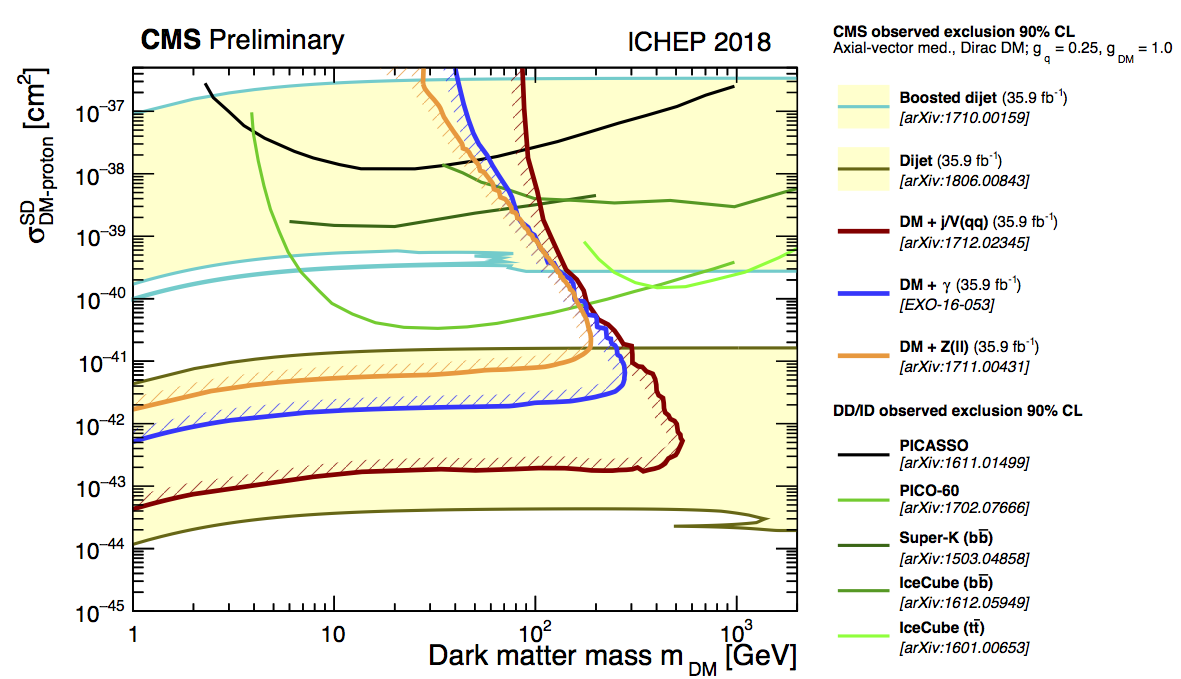
\includegraphics[]{Analysis/Figures/limits/SD_CMSDD_Summary.png}
  }
  \caption{
    Exclusion contours in the $\sigma_{\text{SD}}$--\mdm\ plane for the latest dark matter searches.
    The blue contour shows the results from this thesis, while the red and orange contours show the results from similar searches with jets and vector bosons.
    The light yellow bands show the results from dijet searches for heavy mediators and the green contours show the results from direct and indirect detection searches.
    Citations for all results are given in the figure.
    }
    \label{fig:final_plot}
\end{figure}

During Run 2 of the LHC, a total of 180\fbinv\ of proton-proton collisions data was collected.
This quintupling of the dataset size greatly reduces the statistical uncertainties inherent to the simultaneous fit methodology used in this thesis, promising further increases in discovery potential.
Additionally, the larger dataset allows for new techniques and probes of more exotic models of dark matter.
The coming decade should provide to be an exciting time for the study of dark matter.
